\documentclass[a4paper,10pt]{article}
\usepackage{graphicx}
\usepackage{caption}
\usepackage{enumitem}
\usepackage{multicol}
\usepackage{mathtools}
\usepackage{amsmath,amsthm,amssymb,cancel,bm}
\usepackage{floatrow}
\setcounter{tocdepth}{2}
\usepackage{geometry}
\geometry{total={210mm,297mm},
left=25mm,right=25mm,%
bindingoffset=0mm, top=20mm,bottom=20mm}
\newcommand{\linia}{\rule{\linewidth}{0.5pt}}
\AtBeginDocument{%
   \setlength\abovedisplayskip{-3pt}
   \setlength\belowdisplayskip{5pt}}

\usepackage{hyperref}
\hypersetup{colorlinks=true,linkcolor=blue,citecolor=green,filecolor=cyan,urlcolor=magenta}

% my own titles
\makeatletter
\renewcommand{\maketitle}{
\begin{center}
\vspace{2ex}
{\huge \textsc{\@title}}
\vspace{1ex}
\\
\linia\\
\@author
\vspace{4ex}
\end{center}
}
\makeatother

% custom footers and headers
\usepackage{fancyhdr,lastpage}
\pagestyle{fancy}
\lhead{}
\chead{}
\rhead{}
\renewcommand{\headrulewidth}{0pt}
\lfoot{General Qualifying Exam Solutions}
\cfoot{}
\rfoot{Page \thepage\ /\ \pageref*{LastPage}}

% --------------------------------------------------------------
%
%                           TITLE PAGE
%
% --------------------------------------------------------------

\begin{document}
\hfill{\textit{Last modified \today}}
\title{General Qualifying Exam Solutions: Galactic Astronomy}
\author{Jessica Campbell, Dunlap Institute for Astronomy \& Astrophysics (UofT)}
\date{\today}
\maketitle

\tableofcontents



% --------------------------------------------------------------
%
%
%                              GALACTIC 
%
%
% --------------------------------------------------------------

\newpage
\section{Galactic Astronomy}

% --------------------------------------------------------------
%               1. 
% --------------------------------------------------------------

\subsection{Question 1}

What is a stellar Initial Mass Function (IMF)? Sketch it. Give a couple of examples of simple parametric forms used to describe the IMF, such as the Chabrier, Kroupa, or Salpeter functions.

\subsubsection{Short answer}

Answer.

\subsubsection{Additional context}

The IMF is perhaps the single most important distribution in stellar and galactic astrophysics. Almost all inferences that go from light to physical properties for unresolved stellar populations rely on an assumed form of the IMF, as do almost all models of galaxy formation and the ISM.

{\noindent}If we sum over the stars formed in a large star-forming region (e.g., the Orion Nebula Cluster), we can discuss the distribution of initial stellar masses -- the \textbf{initial mass function}, or IMF. Beginning with the pioneering work of Salpeter (1955), there have been many studies of the IMF in different regions of the Milky Way, and in other galaxies. There is no reason to think that the IMF should be universal, yet it shows remarkable uniformity from region to region. There may be systematic variations in the IMF depending on environmental conditions, but the variations are surprisingly small. It is difficult to determine the IMF at the high-mass end because massive stars are rare, and at the low-mass end because low-mass stars are faint. Nevertheless, for $0.01$ to $50\,{\rm M_\odot}$, there is reasonable agreement between different studies.

{\noindent}Figure \ref{fig:KroupaChabrier} shows two recent estimates (Kroupa 2001; Chabrier 2003) for the IMF in the disk of the MW. For $M\gtrsim1\,{\rm M_\odot}$, the observations are consistent with a power law $\mathrm{d}N/\mathrm{d}M\propto M^{-2.3}$, very close to the slope $\mathrm{d}N/\mathrm{d}M\propto M^{-2.35}$ originally found in the pioneering study by Salpeter (1955). The Kroupa and Chabrier estimates for the IMF differ only in detail. While appreciable numbers of low-mass stars are formed, the mass per logarithmic mass interval peaks near $\sim0.5-1\,{\rm M_\odot}$. Table \ref{table:chabrier} provides some useful integral properties of the IMF. For example, for a total star formation rate $\dot{M}$, the rate of formation of $M>8\,{M_\odot}$ stars is $\dot{M}\times0.2118/19.14\,{\rm M_\odot}$. If $M>8\,{M_\odot}$ stars become Type II supernovae, then the Milky Way star formation rate $\sim1.3\,{\rm M_\odot\,yr^{-1}}$corresponds to a Type II SN rate $0.014\,{\rm yr^{-1}}=1/70\,{\rm yr}$.

\begin{figure}[h]
    \floatbox[{\capbeside\thisfloatsetup{capbesideposition={right,top},capbesidewidth=4cm}}]{figure}[\FBwidth]
    {\caption{\footnotesize{$M\mathrm{d}N/\mathrm{d}lnM$, the mass formed per logarithmic interval in stellar mass $M$, for IMFs of Kroupa (2001) and Chabrier (2003), normalized to the value at $M=1\,{M_\odot}$. Figure taken from Draine (2011).}}
    \label{fig:KroupaChabrier}}
    {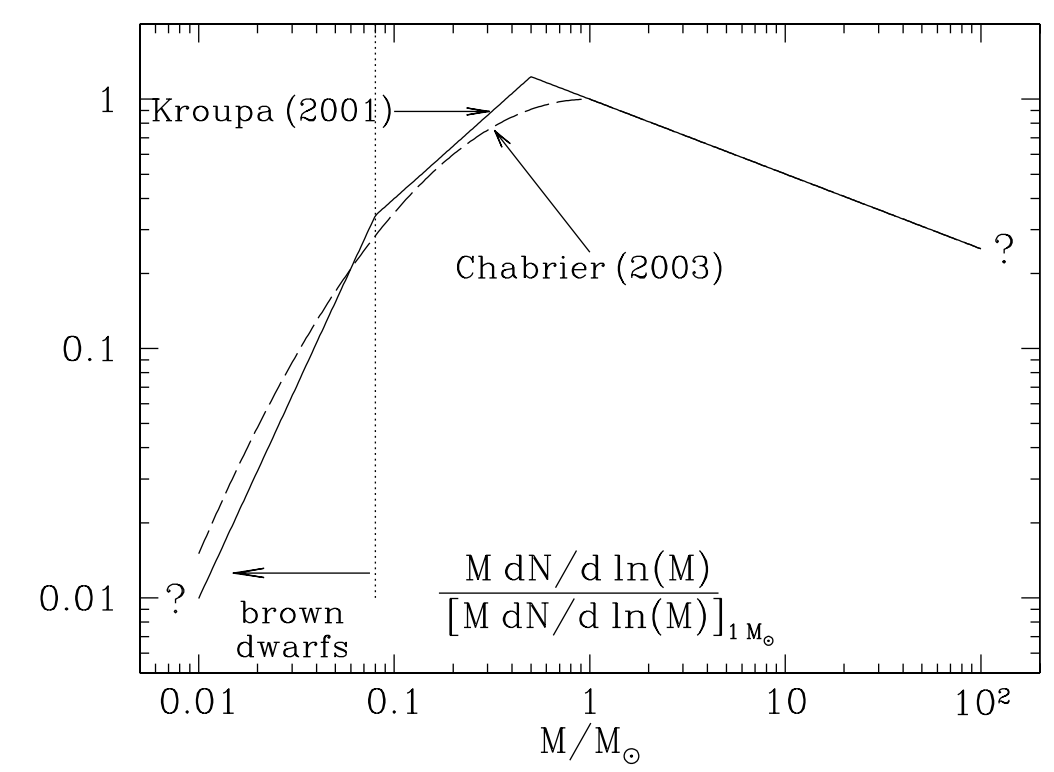
\includegraphics[width=10cm]{figures/KroupaChabrier.png}}
\end{figure}

{\noindent}Since the observable signatures for star formation are obtained only from massive stars, their formation rate needs to be extrapolated to lower masses to obtain the full SFR by assuming an IMF. Typically, a Salpeter-IMF is chosen between $0.1\,M_\odot\leq M\leq 100\,M_\odot$. However, there are clear indications that the IMF may be flatter for $M\lesssim1\,M_\odot$ than described by the Salpeter law, and several descriptions for such modified IMFs have been developed over the years, mainly based on observations and interpretation of star-forming regions in our MW or in nearby galaxies. The total stellar mass, obtained by integration over the IMF, is up to a factor of $\sim2$ lower in these modified IMFs than for the Salpeter IMF. Thus, this factor provides a characteristic uncertainty in the determination of the SFR from observations; a similar, though somewhat smaller uncertainty applies to the stellar mass density whose estimation also is mainly based on the more massive stars of a galaxy which dominate the luminosity. Furthermore, the IMF need not be universal, but may in principle vary between different environments, or depend on the metallicity of the gas from which stars are formed. Whereas there has not yet been unambiguous evidence for variations of the IMF, this possibility must always be taken into account.

\begin{table}[t]
    \centering
    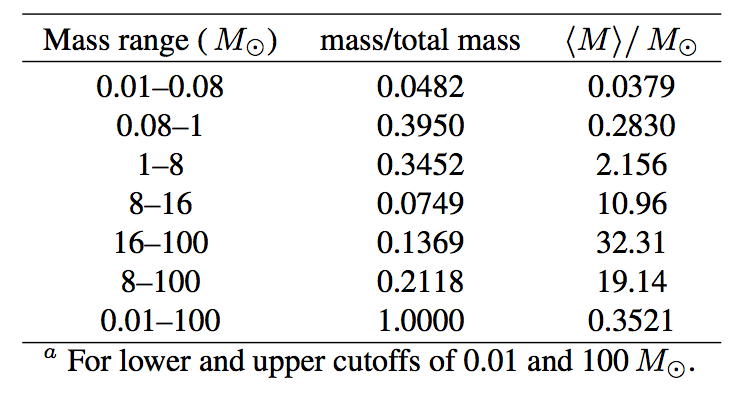
\includegraphics[width=10cm]{figures/ChabrierTable.png}
    \caption{\footnotesize{Some Properties of the Chabrier (2003) IMF$^a$. Table taken from Draine (2011).}}
    \label{table:chabrier}
\end{table}

{\noindent}As with theoretical models of the star formation rate, there is at present no completely satisfactory theory for the origin of the IMF, just different ideas that do better or worse at various aspects of the problem. To recall, the things we would really like to explain most are (1) the slope of the power-law at high masses, and (2) the location of the peak mass. We would also like to explain the little-to-zero variation in these quantities with galactic environment. Furthermore, we would like to explain the origin of the distribution of binary properties.

{\noindent}\textbf{The power-law tail}: Let us begin by considering the power-law tail at high masses, $\mathrm{d}N/\mathrm{d}M\propto M-\alpha$ with $\alpha\approx2.3$. There are two main classes of theories for how this power-law tail is set: competitive accretion, and turbulence. Both are scale-free processes that could plausibly produce a power-law distribution of masses comparable to what is observed.

{\noindent}\textit{Competitive accretion}: One hypothesis for how to produce a power-law mass distribution is to consider what will happen in a region where a bunch of small ``seed'' stars are formed, but then begin to accrete at a rate that is a function of their current mass. Quantitatively, and for simplicity, suppose that every star accretes at a rate proportional to some power of its current mass, i.e.,

\begin{align*}
    \frac{dM}{dt} \propto M^\eta ~ [{\rm M_\odot\,yr^{-1}}].
\end{align*}

{\noindent}If we start with a mass $M_0$ and accretion rate $\dot{M}_0$ at time $t_0$, this ODE is easy to solve for the mass at later times. We get

\begin{equation*}
M(t) = M_o
\left\{
\begin{aligned}
[1-(\eta-1)\tau]^{1/(1-\eta)} ~ [{\rm M_\odot}], ~~~~~& \mathrm{if}\,\eta\neq1 \\
\exp(\tau) ~ [{\rm M_\odot}], ~~~~~& \mathrm{if}\,\eta=1
\end{aligned}
\right.
,
\end{equation*}

{\noindent}where $\tau=t/(M_0/\dot{M}_0)$ is the time measured in units of the initial mass-doubling time. The case for $\eta=1$ is the usual exponential growth, and the case for $\eta>1$ is even faster, running away to infinite mass in a finite amount of time $\tau=1/(\eta-1)$.

{\noindent}Now suppose that we start with a collection of stars that all begin at mass $M_0$, but have slightly different values of $\tau$ at which they stop growing, corresponding either to growth stopping at different physical times from one star to another, to stars stopping at the same time but having slightly different initial accretion rates $\dot{M}_0$, or some combination of both. What will the mass distribution of the resulting population be? If $dN/d\tau$ is the distribution of stopping times, then we will have

\begin{align*}
    \frac{dN}{d\tau} \propto \frac{dN/d\tau}{dM/\tau}M(\tau)^{-\eta}\frac{dN}{d\tau} ~ [{\rm dimensionless}].
\end{align*}

{\noindent}Thus the final distribution of masses will be a power-law in mass, with index $-\eta$, going from $M(\tau_\mathrm{min})$ to $M(\tau_\mathrm{max})$. Thus a power-law distribution naturally results.

{\noindent}The index of this power-law will depend on the index of the accretion law, $\eta$. What should this be? In the case of a point mass accreting from a uniform, infinite medium at rest, the accretion rate onto a point mass was worked out by Hoyle; Bondi generalized to the case of a moving medium. In either case, the accretion rate scales as $\dot{M}\propto M^2$, so if this process describes how stars form, then the expected mass distribution should follow $dN/dM\propto M^{-2}$, not so far from the actual slope of $-2.3$ that we observe. A number of authors have argued that this difference can be made up by considering the effects of a crowded environment, where the feeding regions of smaller stars get tidally truncated, and thus the growth law winds up begin somewhat steeper than $\dot{M}\propto M^2$.

{\noindent}This is an extremely simple model, requiring no physics but hydrodynamics and gravity, and thus it is easy to simulate. Simulations done based on this model do sometimes return a mass distribution that looks much like the IMF, as illustrated in Figure \ref{fig:imf}. However, this appears to depend on the choice of initial conditions. Generally speaking, one gets about the right IMF if one stars with something with a viral ratio $\alpha_\mathrm{vir}\sim1$ and no initial density structure, just velocities. Simulations that start with either super-virial or sub-virial initial conditions, or that begin with turbulent density structures, do not appear to grow as predicted by competitive accretion.

\begin{figure}[t]
    \floatbox[{\capbeside\thisfloatsetup{capbesideposition={right,top},capbesidewidth=4cm}}]{figure}[\FBwidth]
    {\caption{\footnotesize{The IMF measured in a simulation of the collapse of a $500\,{\rm M_\odot}$ initially uniform density cloud (Bate, 2009a). The single-hatched histogram shows all objects in the simulation, while the double-hatched one shows objects that have stopped accreting. Figure taken from Draine (2011).}}
    \label{fig:imf}}
    {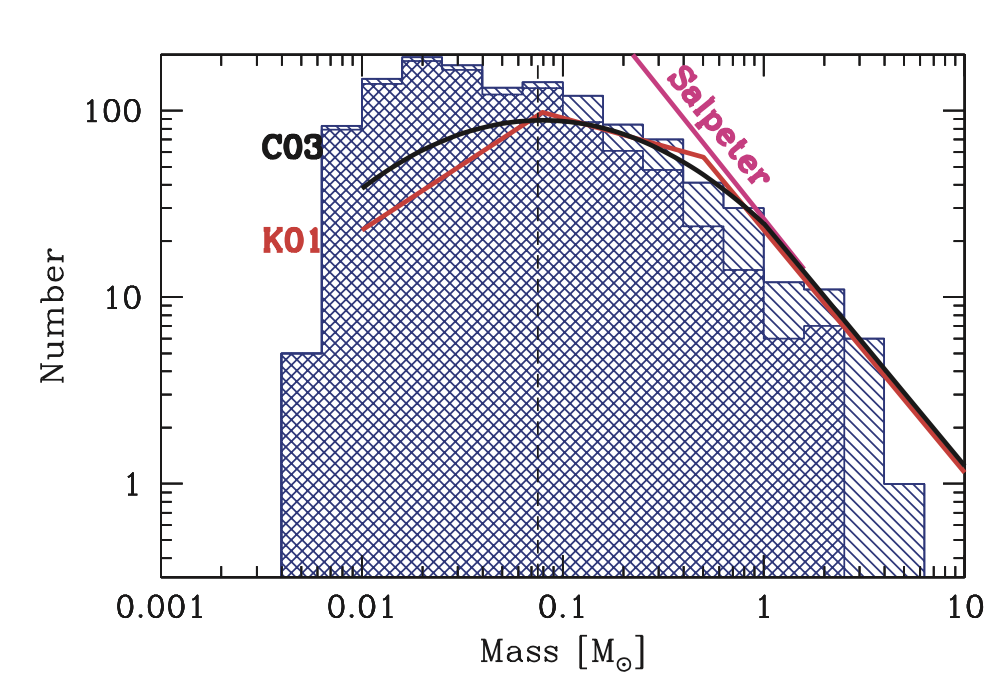
\includegraphics[width=12cm]{figures/IMF.png}}
\end{figure}

{\noindent}Another potential problem with this model is that it only seems to work in environments where there is no substantial feedback to drive the turbulence or eject the gas. In simulations where this is not true, there appears to be no competitive accretion. The key issue is that competitive accretion seems to require a global collapse where all the stars fall together into a region where they can compete, and this is hard to accomplish in the presence of feedback.

{\noindent}\textit{Turbulent fragmentation}: A second class of models for the origin of the power-law slope is based on the physics of turbulence. The first of these models was proposed by Padoan et al. (1997), and there have been numerous refinements since. The basic assumption in the turbulence models is that the process of shocks repeatedly passing through an isothermal medium leads to a broad range of density distributions, and that stars form wherever a local region happens to be pushed to the point where it becomes self-gravitating. We then proceed as follows. Suppose we consider the density field smoothed on some size scale $\ell$. The mass of an object of density $\rho$ in this smoothed field is

\begin{align*}
    M \sim \rho\ell^3 ~ [{\rm M_\odot}],
\end{align*}

{\noindent}and the total mass of objects with characteristic density between $\rho$
and $\rho+d\rho$ is

\begin{align*}
    dM_\mathrm{tot} \sim \rho p(\rho)d\rho ~ [{\rm M_\odot}],
\end{align*}

{\noindent}where $p(\rho)$ is the density PDF. Then the total number of objects in the mass range from $M$ to $M+dM$ on size scale $\ell$ can be obtained just by dividing the total mass of objects at a given density by the mass per object, and integrating over the density PDF on that size scale,

\begin{align*}
    \frac{dN_\ell}{dM} = \frac{dM_\mathrm{tot}}{M} \sim \ell^{-3} \int p(\rho)d\rho ~ [{\rm dimensionless}].
\end{align*}

{\noindent}Not all of these structures will be bound. To filter out the ones that are, we can impose a density threshold. We assert that an object will be bound only if its gravitational energy exceeds its kinetic energy, that is, only if the density exceeds a critical value given by

\begin{align*}
    \frac{GM^2}{\ell} \sim M\sigma_v(\ell)^2 ~ [{\rm J}] ~~~~~ \Rightarrow ~~~~~ \rho_\mathrm{crit} \sim \frac{\sigma_v(\ell)^2}{G\ell^2} ~ [{\rm g\,cm^{-3}}],
\end{align*}

{\noindent}where $\sigma_v(\ell)$ is the velocity dispersion on size scale $\ell$, which we take from the linewidth-size relation, $\sigma_v(\ell) = c_s\sqrt{(\ell/\ell_s)}$. Thus we have a critical density

\begin{align*}
    \rho_\mathrm{crit} \sim \frac{c_s^2}{G\ell_s\ell} ~ [{\rm g\,cm^{-3}}],
\end{align*}

{\noindent}and this forms a lower limit on the integral.

{\noindent}There are two more steps in the argument. One is simple: just integrate over all length scales to get the total number of objects. That is, 

\begin{align*}
    \frac{dN}{dM} \propto \frac{dN_\ell}{dM}d\ell ~ [{\rm M_\odot^{-1}}]. 
\end{align*}

{\noindent}The second is that we must know the functional form of $p(\rho)$ for the smoothed density PDF. One can get this in a couple of different ways, but there isn't a fully rigorous calculation. Hopkins get it by assuming that the PDF is log-normal smoothed on all scales with a dispersion that is an integral over the dispersions on smaller scales. Hennebelle \& Chabrier, in their model, assume that the density power spectrum is a power-law, and derive the density PDF from that. The assumptions yield similar but not identical results. 

{\noindent}At this point we will simply assert that one can evaluate all the integrals to get an IMF. The result clearly depends only on two dimensional quantities: the sound speed $c_s$ and the sonic length $\ell_s$. However, at masses much greater than the sonic mass $M_s \approx c_s^2\ell_s/G$, the result is close to a power-law with approximately the right index. Figure \ref{fig:imfmodel} shows an example prediction.

\begin{figure}[t]
    \floatbox[{\capbeside\thisfloatsetup{capbesideposition={right,top},capbesidewidth=4cm}}]{figure}[\FBwidth]
    {\caption{\footnotesize{The IMF predicted by an analytic model of turbulent fragmentation by Hopkins (2012). Figure taken from Draine (2011).}}
    \label{fig:imfmodel}}
    {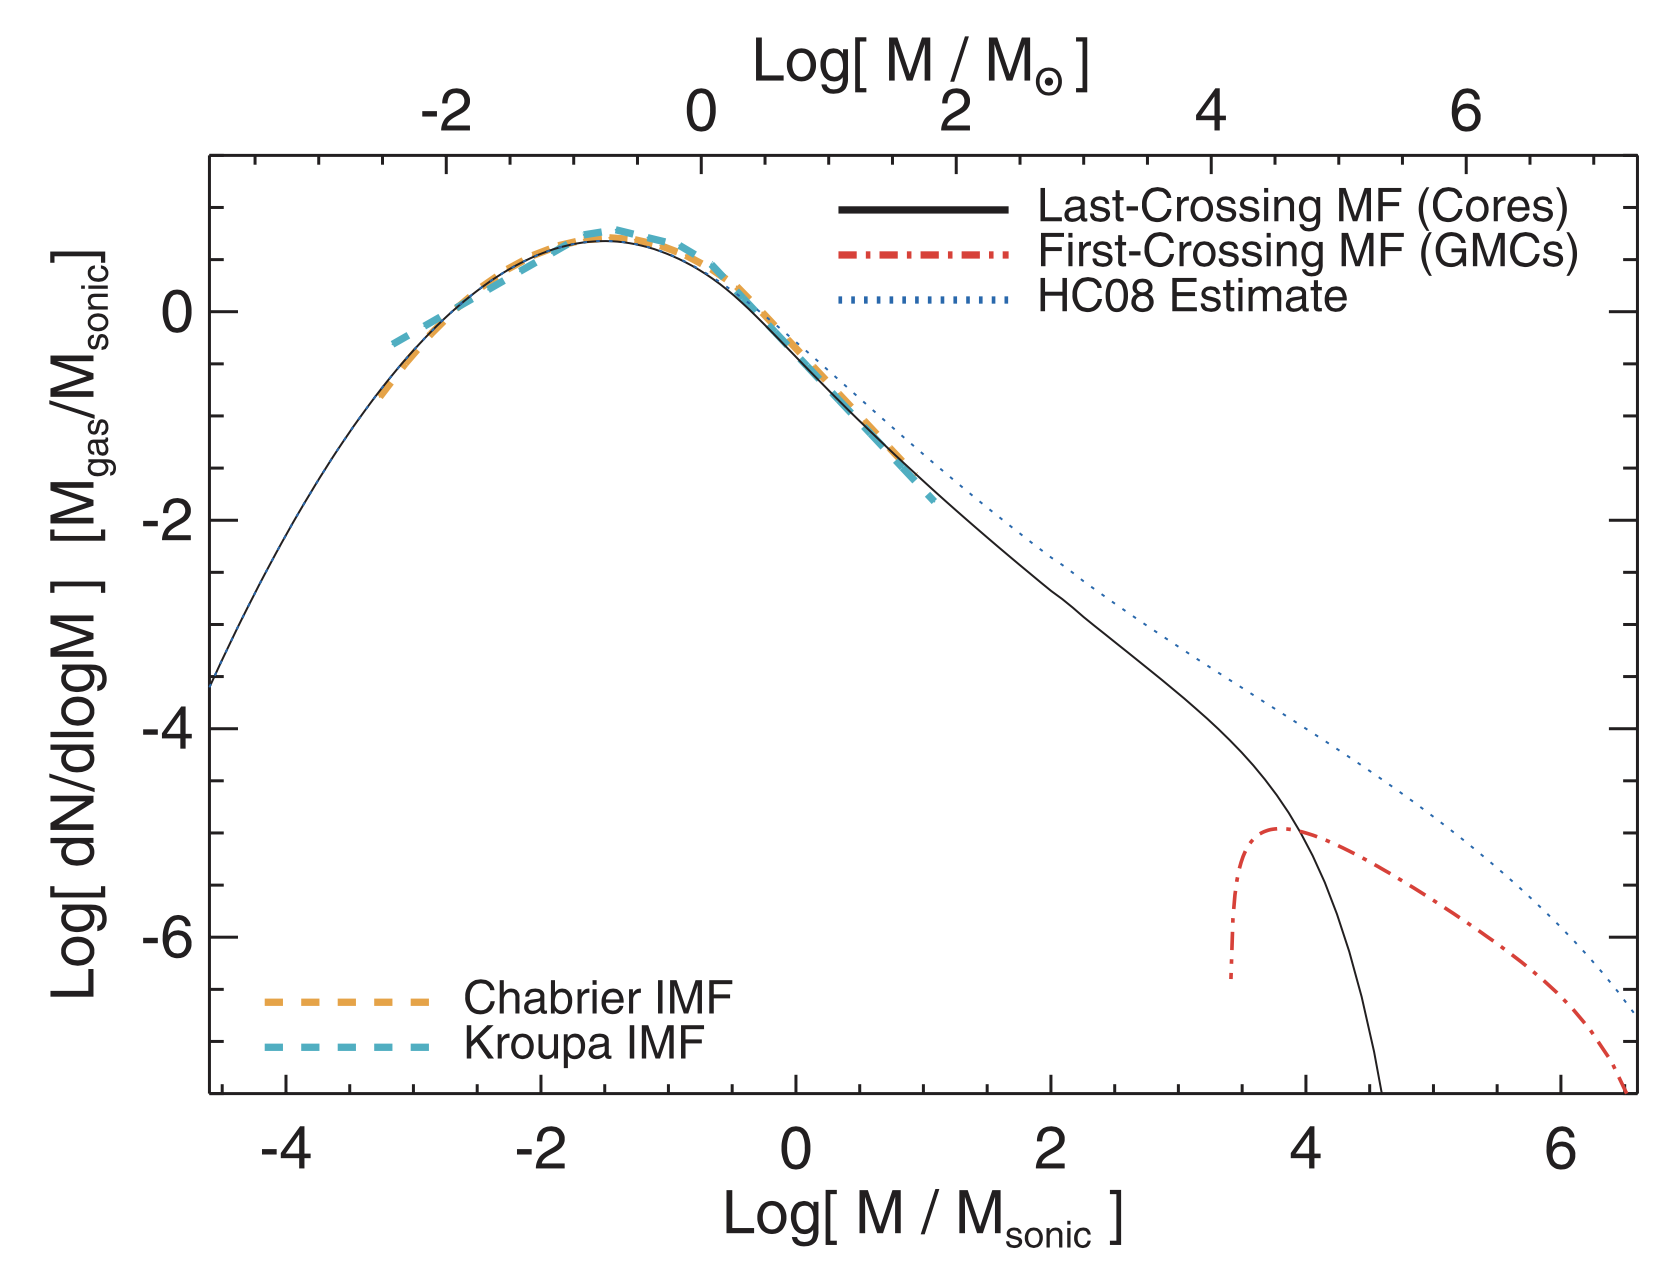
\includegraphics[width=12cm]{figures/IMFmodel.png}}
\end{figure}

{\noindent}As with the competitive accretion model, this hypothesis encounters certain difficulties. First, there is the technical problem that the choice of smoothed density PDF estimate is not at all rigorous, and there are noticeable differences between on how the choice is made. Second, the dependence on the sonic length is potentially problematic, because real molecular clouds do not really have constant sonic lengths. Regions of massive star formation are observed to be systematically more turbulent.

{\noindent}Third, the theory does not address the question of why gravitationally-bound regions don’t sub-fragment as they collapse. Finally, the model has trouble explaining the IMF peak, for the exact same reason as competitive accretion.

{\noindent}\textbf{The peak of the IMF}: A power-law is scale-free, but the peak has a definite mass scale. This mass scale is one basic observable that any theory of star formation must be able to predict. This immediately tells us something about the physical processes that must be involved. We have thus far thought of molecular clouds as consisting mostly of isothermal, turbulent, magnetized, self-gravitating gas. However, we can show that there must be additional processes beyond these at work in setting a peak mass.

{\noindent}We can see this in a few ways. First we'll demonstrate it in a more intuitive but not rigorous manner, and then we can demonstrate it rigorously. The intuitive arguments is as follows. In the system we have described, there are four energies in the problem: thermal energy, bulk kinetic energy, magnetic energy, and gravitational potential energy. From these energies we can define three dimensionless ratios, and the behavior of the system will be determined by these three ratios. As an example, we might define

\begin{align*}
    \mathcal{M}=\frac{\sigma_v}{c_s} ~ [{\rm dimensionless}] ~~~~~ \beta=\frac{8\pi\rho c_c^2}{b^2} ~ [{\rm dimensionless}] ~~~~~ n_J=\frac{\rho L^2}{c_s^3/\sqrt{G^3\rho}} ~ [{\rm dimensionless}].
\end{align*}

{\noindent}The ratios describe the ratio of kinetic to thermal energy, the ratio of thermal to magnetic energy, and the ratio of thermal to gravitational energy. (This last quantity is called the Jeans number: it is the ratio of the cloud mass to the Jeans mass.) Other ratios can be derived from these, e.g., the Alfv\'enic Mach number $\mathcal{M}=\mathcal{M}\sqrt{\beta/2}$ is the ratio of the kinetic to magnetic energy.

{\noindent}Now notice the scalings of these numbers with density $\rho$, velocity dispersion $\sigma_v$, magnetic field strength $B$, and length scale $L$:

\begin{align*}
    \mathcal{M}\propto\sigma_v ~ [{\rm dimensionless}] ~~~~~ \beta\propto\rho B^{-2} ~ [{\rm dimensionless}] ~~~~~ n_J\propto\rho^{3/2}L^3 ~ [{\rm dimensionless}].
\end{align*}

{\noindent}Notice that if we scale the problem by $\rho\rightarrow x\rho$, $L\rightarrow x^{-1/2}L$, $B\rightarrow x^{1/2}B$, all of these dimensionless numbers remain fixed. Thus the behavior of two systems, one with density a factor of $x$ times larger than the other one, length a factor of $x^{-1/2}$ smaller, and magnetic field a factor of $x^{1/2}$ stronger, are simply rescaled versions of one another. If the first system fragments to make a star out of a certain part of its gas, the second system will too. Notice, however, that the masses of those stars will not be the same! The first star will have a mass that scales as $\rho L^3$, while the second will have a mass that scales as $(x\rho)(x^{-1/2}L)^3=x^{-1/2}\rho L^3$.

{\noindent}We learn from this an important lesson: isothermal gas is scale-free. If we have a model involving only isothermal gas with turbulence, gravity, and magnetic fields, and this model produces stars of a given mass $M_*$, then we can rescale the system to obtain an arbitrarily different mass. Explaining the IMF peak requires appealing to some physics beyond that of isothermal, magnetized turbulence plus self-gravity. This immediately shows that the competitive accretion and turbulence theories we outlined to explain the power-law tail of the IMF cannot be adequate to explaining the IMF peak, at least not by themselves. Something must be added, and models for the origin of the IMF peak can be broadly classified based on what extra physics they choose to add.

{\noindent}\textbf{The outer scale of turbulence}: One option is hypothesize that the IMF is set at the outer scale of the turbulence, where the molecular clouds join to the atomic ISM (in a galaxy like the MW), or on sizes of the galactic scale-height (for a molecule-dominated galaxy). Something in this outer scale picks out the characteristic mass of stars at the IMF peak.

{\noindent}This hypothesis comes in two flavors. The simplest is that characteristic mass is simply set by the Jeans mass at the mean density of the cloud, so that

\begin{align*}
    M_\mathrm{peak} \propto \frac{c_s^3}{\sqrt{G^3\bar{\rho}}} ~ [{\rm M_\odot}].
\end{align*}

{\noindent}While simple, this hypothesis immediately encounters problems. Molecular clouds have about the same temperature everywhere, but they do not all have the same density -- indeed, the density should vary with cloud mass as $M^{1/2}$. Thus at face value this hypothesis would seem to predict a factor of $\sim3$ difference in characteristic peak mass between $10^4$ and $10^6\,{\rm M_\odot}$ clouds in the MW. This is pretty hard to reconcile with observations. The problem is even worse if we think about other galaxies, where the range of density variation is much greater and thus the predicted IMF variation is too. One can hope for a convenient cancellation, whereby an increase in the density is balanced by an increase in temperature, but this seems to require a coincidence.

{\noindent}A somewhat more refined hypothesis, which is adopted by all the turbulence models, is that the IMF peak is set by the sound speed and the normalization of the linewidth-size relation. As discussed above, in the turbulence models the only dimensional free parameters are $c_s$ and $\ell_s$, and from them one can derive a mass in only one way:

\begin{align*}
    M_\mathrm{peak} \propto \frac{c_s^2\ell_s}{G} ~ [{\rm M_\odot}].
\end{align*}

{\noindent}Hopkins calls this quantity the sonic mass, but it’s the same thing as the characteristic masses in the other models.

{\noindent}This value can be expressed in a few ways. Suppose that we have a cloud of characteristic mass $M$ and radius $R$. We can write the velocity dispersion in terms of the virial parameter:

\begin{align*}
    \alpha_\mathrm{vir} \sim \frac{\sigma_vR}{GM} ~ [{\rm dimensionless}].
\end{align*}

{\noindent}This is the velocity dispersion on the outer scale of the cloud, so we can also define the Mach number on this scale as

\begin{align*}
    \mathcal{M} = \frac{\sigma_v}{c_s} \sim \sqrt{\alpha_\mathrm{vir}\frac{GM}{Rc_s^2}} ~ [{\rm dimensionless}].
\end{align*}

{\noindent}The sonic length is just the length scale at which $\mathcal{M}\sim1$, so if the velocity dispersion scales with $\ell^{1/2}$, then we have

\begin{align*}
    \ell_s \sim \frac{R}{\mathcal{M}^2} \sim \frac{c_s^2}{\alpha_\mathrm{vir}G\Sigma} ~ [{\rm pc}].
\end{align*}

{\noindent}Substituting this in, we have

\begin{align*}
    M_\mathrm{peak} \sim \frac{c_s^4}{\alpha_\mathrm{vir}G^2\Sigma} ~ [{\rm M_\odot}],
\end{align*}

{\noindent}and thus the peak mass simply depends on the surface density of the cloud. We can obtain another equivalent expression by noticing that

\begin{align*}
    \frac{M_J}{\mathcal{M}} \sim \frac{c_s^3}{\sqrt{G^3\bar{\rho}}} \sqrt{\frac{Rc_s^2}{\alpha_\mathrm{vir}GM}} \sim \frac{c_s^4}{\alpha_\mathrm{vir}G^2\Sigma} \sim M_\mathrm{peak} ~ [{\rm M_\odot}].
\end{align*}

{\noindent}Thus, up to a factor of order unity, this hypothesis is also equivalent to assuming that the characteristic mass is simply the Jeans mass divided by the Mach number.

{\noindent}An appealing aspect of this argument is that it naturally explains why molecular clouds in the MW all make stars at about the same mass. A less appealing result is that it would seem to predict that the masses could be quite different in regions of different surface density, and we observe that there are star-forming regions where $\Sigma$ is indeed much higher than the mean of the MW GMCs. This is doubly-true if we extend our range to extragalactic environments. One can hope that this will cancel because the temperature will be higher and thus $c_s$ will increase, but this again seems to depend on a lucky cancellation, and there is no a priori reason why it should.

{\noindent}\textbf{Non-isothermal fragmentation}: The alternative to breaking the isothermality at the outer scale of the turbulence is to relax the assumption that the gas is isothermal on small scales. This has the advantage that it avoids any ambiguity about what constitutes the surface density or linewidth-size relation normalization for a ``cloud''.

{\noindent}The earliest versions of these models were proposed by Larson (2005), and followed up by Jappsen et al. (2005). The basic idea of these models is that the gas in star-forming clouds is only approximately isothermal. Instead, there are small deviations from isothermality, which can pick out preferred mass scales. There are two places where significant deviations from isothermality are expected (Figure \ref{fig:sf_tvsrho}).

\begin{figure}[t]
    \floatbox[{\capbeside\thisfloatsetup{capbesideposition={right,top},capbesidewidth=4cm}}]{figure}[\FBwidth]
    {\caption{\footnotesize{Temperature versus density found in a one-dimensional calculation of the collapse of a $1\,{\rm M_\odot}$ gas cloud, at the moment immediately before a central protostar forms. Figure taken from Draine (2011).}}
    \label{fig:sf_tvsrho}}
    {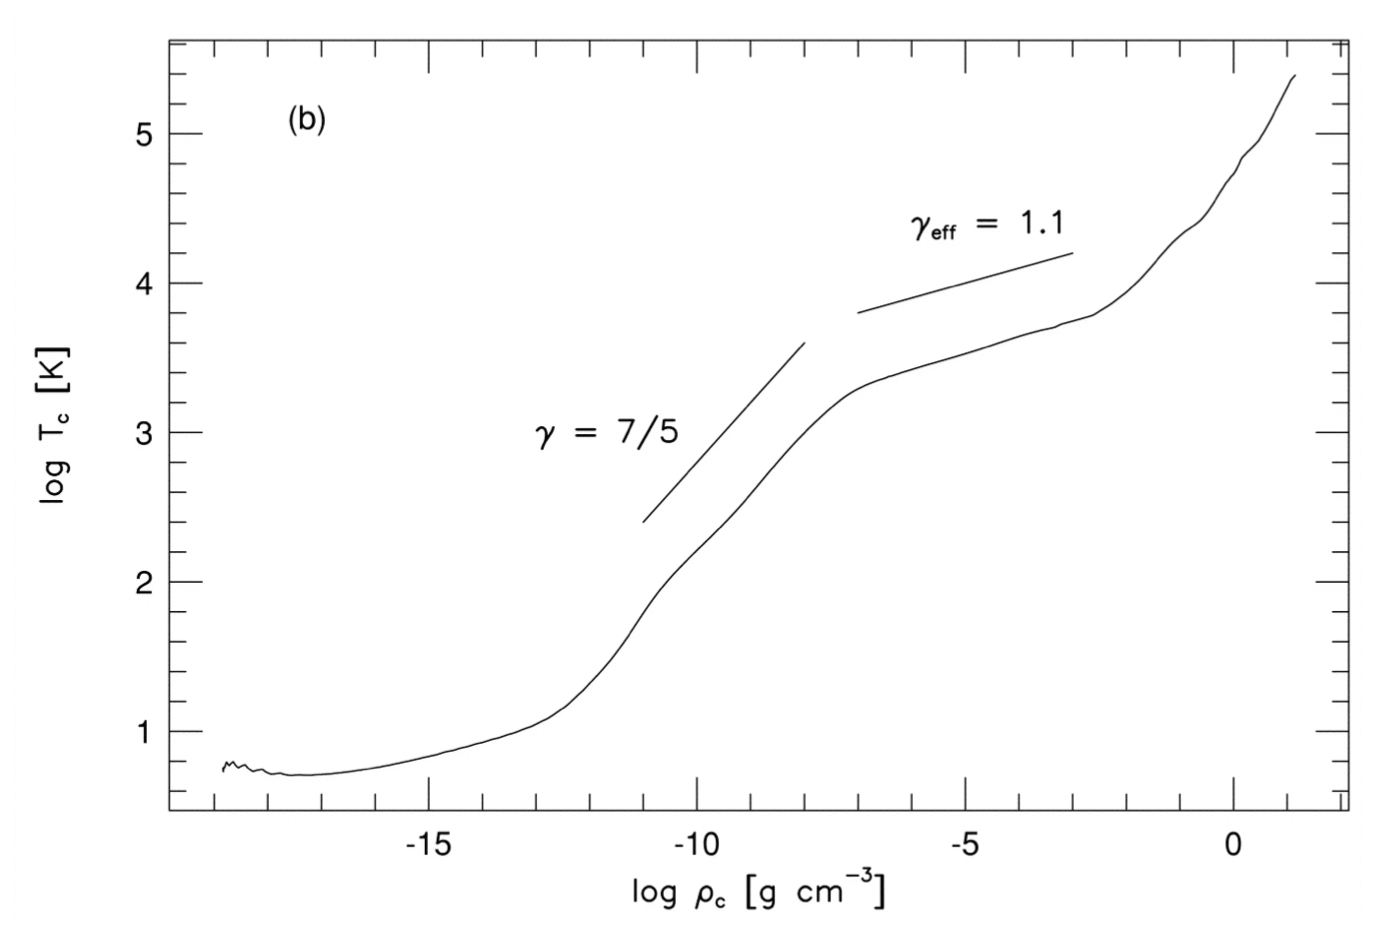
\includegraphics[width=12cm]{figures/SF_TvsRho.png}}
\end{figure}

{\noindent}At low density the main heating source is cosmic rays and UV photons, both of which produce a constant heating rate per nucleus if attenuation is not significant. This is because the flux of CRs and UV photons is about constant, and the rate of energy deposition is just proportional to the number of target atoms or dust grains for them to interact with. Cooling is primarily by lines, either of CO once the gas is mostly molecular, or of C$_\mathrm{II}$ or O where it is significantly atomic.

{\noindent}In both cases, at low density the gas is slightly below the critical density of the line, so the cooling rate per nucleus or per molecule is an increasing function of density. Since heating per nucleus is constant but cooling per nucleus increases, the equilibrium temperature decreases with density. As one goes to higher density and passes the CO critical density this effect ceases. At that point one generally starts to reach densities such that shielding against UV photons is significant, so the heating rate goes down and thus the temperature continues to drop with density.

{\noindent}This begins to change at a density of around $10^{18}\,{g\,cm^{-3}}$, $n\sim10^5--10^6\,{cm^{-3}}$. By this point the gas and dust have been thermally well-coupled by collisions, and the molecular lines are extremely optically thick, so dust is the main thermostat. As long as the gas is optically thin to thermal dust emission, which it is at these densities, the dust cooling rate per molecule is fixed, since the cooling rate just depends on the number of dust grains. Heating at these densities comes primarily from compression as the gas collapses, i.e., it is just $PdV$ work. If the compression were at a constant rate, the heating rate per molecule would be constant. However, the free-fall time decreases with density, so the collapse rate and thus the heating rate per molecule increase with density. The combination of fixed cooling rate and increasing heating rate causes the temperature to begin rising with density. At still higher densities, $10^{13}\,{\rm g\,cm^{-3}}$, the gas becomes optically thick to dust thermal emission. At this point the gas simply acts adiabatically, with all the $PdV$ work being retained, so the heating rate with density rises again.

{\noindent}Larson (2005) pointed out that deviations from isothermality are particularly significant for filamentary structures, which dominate in turbulent flows. It is possible to show that a filament cannot go into runaway collapse if $T$ varies with $\rho$ to a positive number, while it can collapse if $T$ varies as $\rho$ to a negative number. This suggests that filaments will collapse indefinitely in the low-density regime, but that their collapse will then halt around $10^{18}\,{\rm g\,cm^{-3}}$, forcing them to break up into spheres in order to collapse further. The upshot of all these arguments is that the Jeans or Bonnor-Ebert mass one should be using to estimate the peak of the stellar mass spectrum is the one corresponding to the point where there is a changeover from sub-isothermal to super-isothermal.

{\noindent}In other words, the $\rho$ and $T$ that should be used to evaluate $M_J$ or $M_{BE}$ are the values at that transition point. Larson proposes an approximate equation of state to represent the first break in the EOS: Combining all these effects, Larson (2005) proposed a single simple equation of state

\begin{equation*}
T =
\left\{
\begin{aligned}
4.4\rho_{18}^{-0.27} ~ [{\rm K}], ~~~~~& \mathrm{if}\,\rho_{18}<1 \\
4.4\rho_{18}^{0.07} ~ [{\rm K}], ~~~~~& \mathrm{if}\,\rho_{18}\geq1
\end{aligned}
\right.
,
\end{equation*}

{\noindent}where $\rho_{18}=\rho/(10^{18}\,{\rm g\,cm^{-33}})$. Conveniently enough, the Bonnor-Ebert mass at the minimum temperature here is $M_{BE}=0.067\,{\rm M_\odot}$, which is not too far off from the observed peak of the IMF at $M_\mathrm{peak}=0.2\,{\rm M_\odot}$. (The mass at the second break is a bit less promising. At $\rho=10^{13}\,{\rm g\,cm^{13}}$ and $T=10\,{\rm K}$, we have $M_{BE}=7\times10^{-4}\,{\rm M_\odot}$).

{\noindent}Simulations done adopting this proposed equation of state seem to verify the conjecture that the characteristic fragment mass does depend critically on the break on the EOS (Figure \ref{fig:imfmodels}).

\begin{figure}[t!]
    \centering
    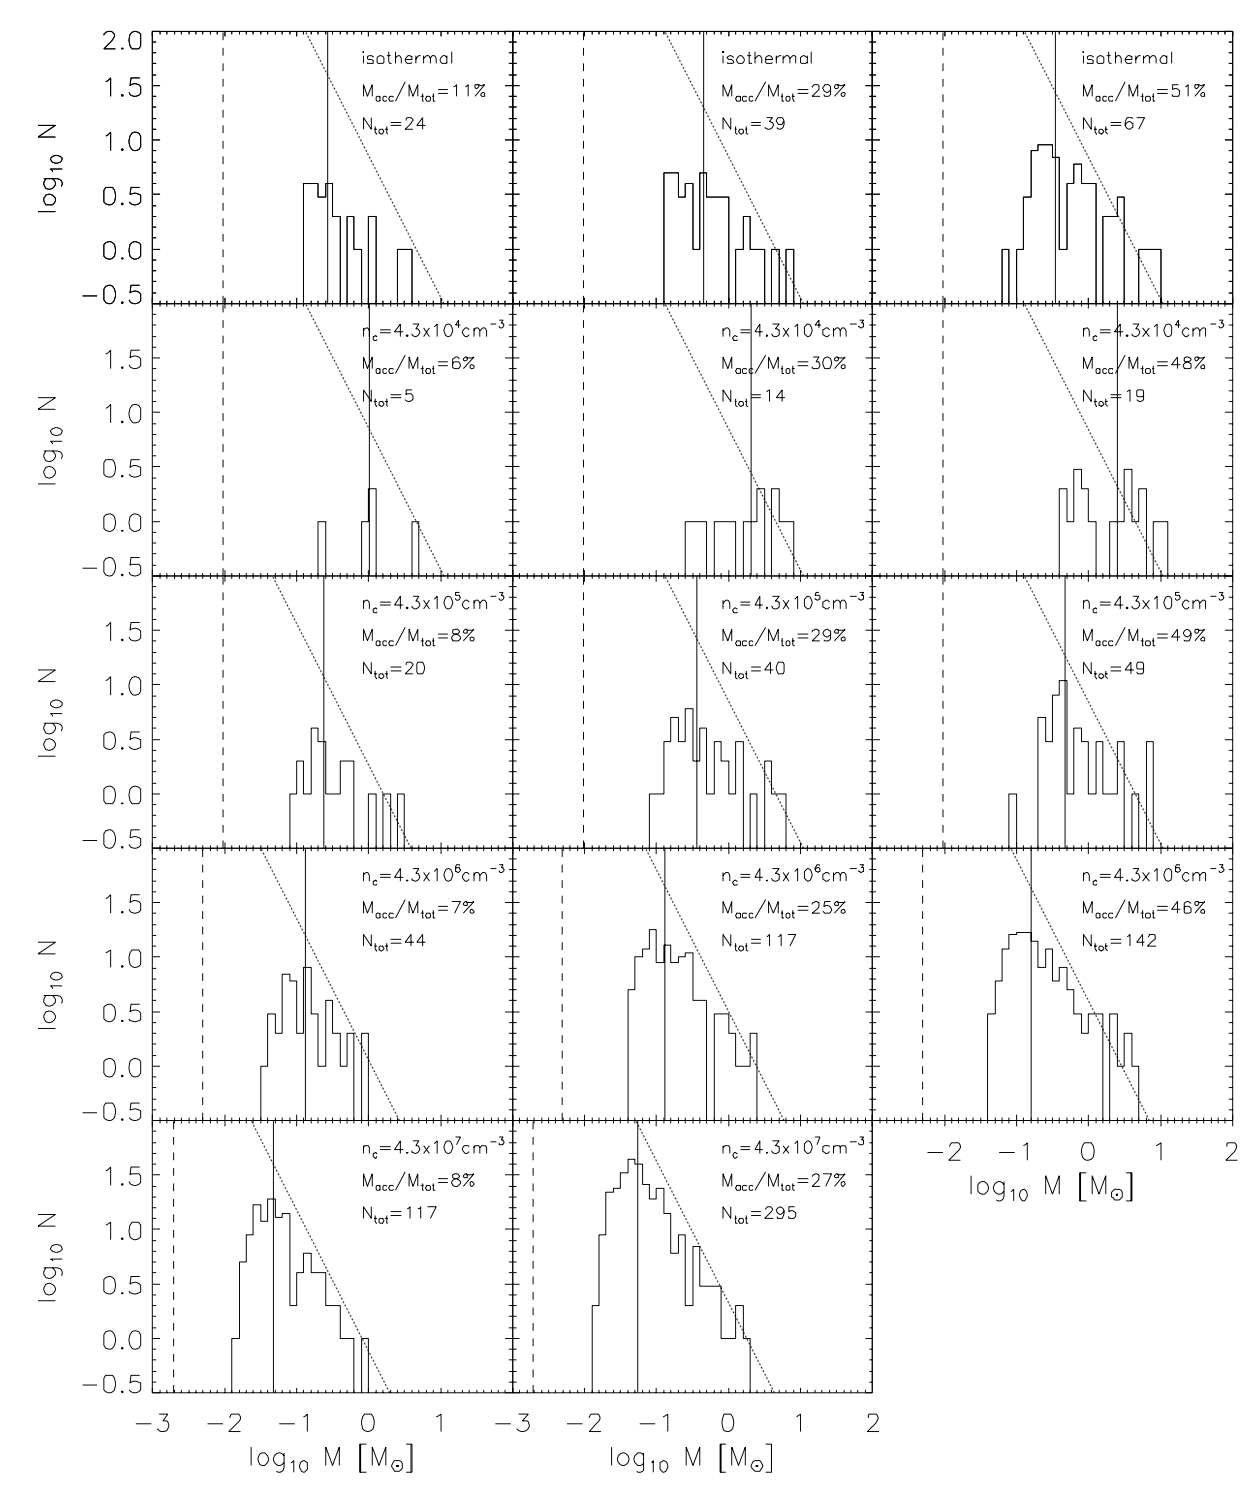
\includegraphics[width=16cm]{figures/IMFmodels.png}
    \caption{\footnotesize{Measured stellar mass distributions in a series of simulations of turbulent fragmentation using non-isothermal EOSs. Each row shows a single simulation, measured at a series of times, characterized by a particular mass in stars as indicated in each panel. Different rows use different EOSs, with the vertical line in each panel indicating the Jeans mass evaluated at the temperature minimum of the equation of state. Histograms show the mass distributions measured for the stars. Figure taken from Draine (2011).}}
    \label{fig:imfmodels}
\end{figure}

{\noindent}While this is a very interesting result, there are two problems. First, the proposed break in the EOS occurs at $n=4\times10^5\,{\rm cm^{-3}}$. This is a fairly high density in a low mass star-forming region, but it is actually quite a low density in more typical, massive star-forming regions. For example, the Orion Nebula cluster (ONC) now consists of $4600\,{M_\odot}$ of stars in a radius of $0.8\,{\rm pc}$, giving a mean density $n=3.7\times10^4\,{\rm cm^{-3}}$. Since the SF efficiency was less than unity and the cluster is probably expanding due to mass loss, the mean density was almost certainly higher while the stars were still forming. Moreover, recall that, in a turbulent medium, the bulk of the mass is at densities above the volumetric mean density. The upshot of all this is that almost all the gas in Orion was probably over Larson (2005)'s break density while the stars were forming. Since Orion managed to form a normal IMF, it's not clear how the break temperature could be relevant.

{\noindent}A second problem is that, in dense regions like the ONC, the simple model proposed by Larson (2005) is a very bad representation of the true temperature structure, because it ignores the effects of radiative feedback from stars. In dense regions the stars that form will heat the gas around them, raising the temperature. Figure \ref{fig:tvsrho_feedback} shows the density-temperature distribution of gas in simulations that include radiative transfer, and that have conditions chosen to be similar to those of the ONC.

\begin{figure}[t]
    \centering
    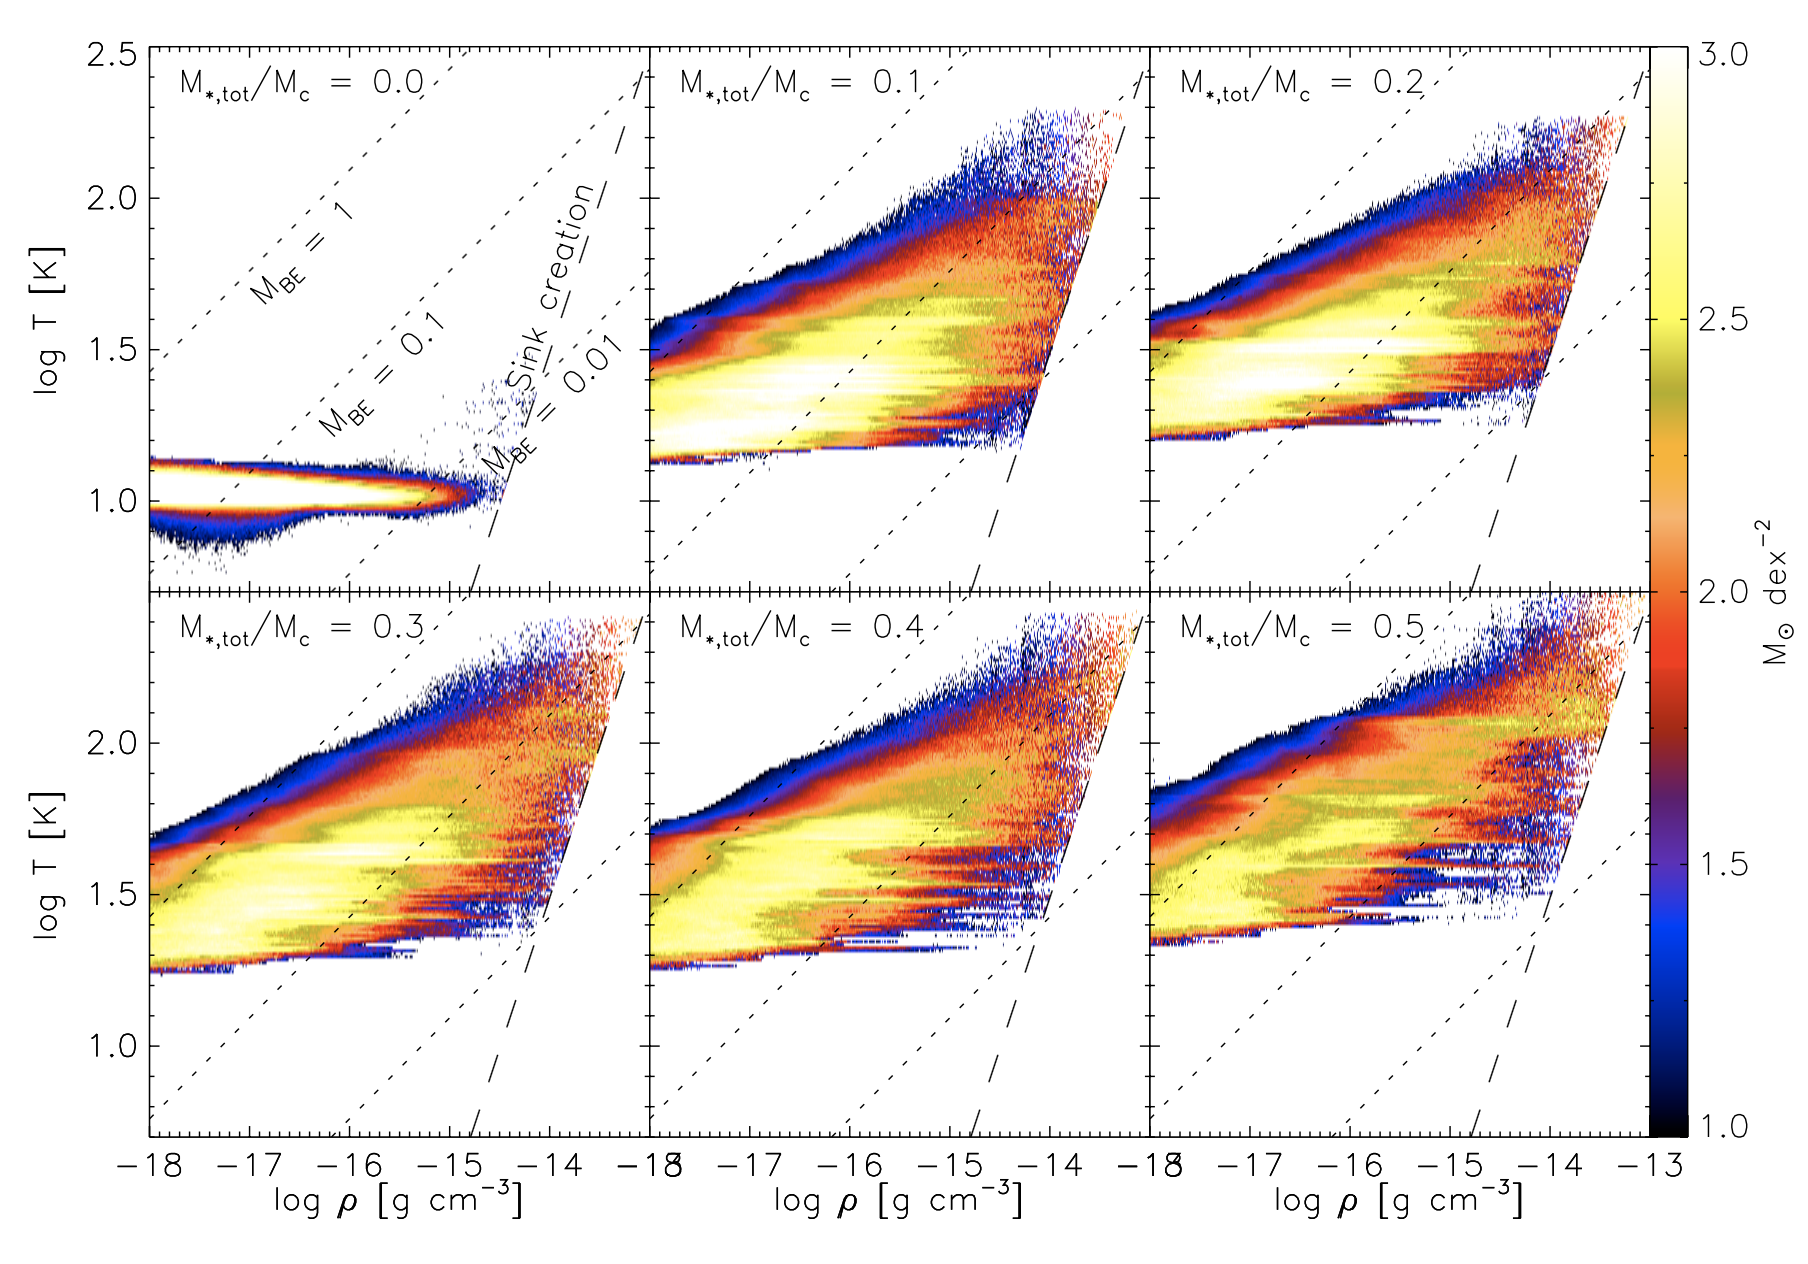
\includegraphics[width=16cm]{figures/TvsRho_feeback.png}
    \caption{\footnotesize{Density-temperature distributions measured from a simulation of the formation of an ONC-like star cluster, including radiative transfer and stellar feedback (Krumholz et al., 2011a). The panels show the distribution at different times in the simulation, characterized by the fraction of mass that has been turned into stars. Doted lines show lines of constant Bonnor-Ebert mass (in ${\rm M_\odot}$), while dashed lines show the threshold for sink particle formation in the simulation. Histograms show the mass distributions measured for the stars. Figure taken from Draine (2011).}}
    \label{fig:tvsrho_feedback}
\end{figure}

{\noindent}These two observations suggest that one can build a model for the IMF around radiative feedback. There are a few numerical and analytic papers that attempt to do so, including Bate (2009b, 2012), Krumholz (2011), and Krumholz et al. (2012b). The central idea for these models is that radiative feedback shuts off fragmentation at a characteristic mass scale that sets the peak of the IMF.

{\noindent}The basic idea is as follows. Suppose that we form a first, small protostellar that radiates at a rate $L$. The temperature of the material at a distance $R$ from it, assuming the gas is optically thick, will be roughly

\begin{align*}
    L\approx 4\pi R^2\sigma T^4 ~ [{\rm erg\,s^{-1}}].
\end{align*}

{\noindent}Now let us compute the Bonnor-Ebert mass using the temperature $T$:

\begin{align*}
    M_{BE} \approx \frac{c_s^3}{\sqrt{G^3\rho}} = \sqrt{\left(\frac{k_BT}{\mu m_HG}\right)^3\frac{1}{\rho}},
\end{align*}

{\noindent}where $\mu=2.33$ is the mean particle mass, and we are omitting the factor of $1.18$ for simplicity. Note that $M_{BE}$ here is a function of $R$. At small $R$, $T$ is large and thus $M_{BE}$ is large, while at larger distances the gas is cooler and $M_{BE}$ falls.

{\noindent}Now let us compare this mass to the mass enclosed within the radius $R$, which is $M=(4/3)\pi R^3\rho$. At small radii, $M_{BE}$ greatly exceeds the enclosed mass, while at large radii $M_{BE}$ is much less than the enclosed mass. A reasonable hypothesis is that fragmentation will be suppressed out to the point where $M\approx M_{BE}$. If we solve for the radius $R$ and mass $M$ at which this condition is met, we obtain

\begin{align*}
    M\approx \left(\frac{1}{36\pi}\right)^{1/10} \left(\frac{k_B}{G\mu m_H}\right)^{6/5} \left(\frac{L}{\sigma}\right)^{3/10} \rho^{-1/5} ~ [{\rm M_\odot}].
\end{align*}

{\noindent}To go further, we need to know the luminosity $L$. The good news is that the luminosity is dominated by accretion, and the energy produced by accretion is simply the accretion rate multiplied by a roughly fixed energy yield per unit mass. In other words, we can write

\begin{align*}
    L \approx \phi\dot{M} ~ [{\rm erg\,s^{-1}}].
\end{align*}

{\noindent}where $\phi=10^{14}\,{\rm erg\,g^{-1}}$, and can in fact be written in terms of fundamental constants. Taking this on faith for now, if we further assume that stars form over a time of order a free-fall time, then

\begin{align*}
    \dot{M}\approx M\sqrt{G\rho} ~ [{\rm M_\odot\,yr^{-1}}],
\end{align*}

{\noindent}and substituting this into the equation for $M$ above and solving gives

\begin{align*}
    M\approx \left(\frac{1}{36\pi}\right)^{1/7} \left(\frac{k_B}{G\mu m_H}\right)^{12/7} \left(\frac{\phi}{\sigma}\right)^{3/7} \rho^{-1/14} = 0.3\left(\frac{n}{100\,{\rm cm^{-3}}}\right)^{-1/14} ~ [{\rm M_\odot}],
\end{align*}

{\noindent}where $n=\rho/(\mu m_H)$. Thus we get a characteristic mass that is a good match to the IMF peak, and that depends only very, very weakling on the ambient density.

{\noindent}Simulations including radiation seem to support the idea that this effect can pick out a characteristic peak ISM mass. The main downside to this hypothesis is that it has little to say by itself about the power-law tail of the IMF. This is not so much a problem with the model as an omission, and a promising area of research seems to be joining a non-isothermal model such as this onto a turbulent fragmentation or competitive accretion model to explain the full IMF.

{\noindent}\textbf{Measuring the IMF}: There are two major strategies for measuring the IMF. One is to use direct star counts in regions where we can resolve individual stars. The other is to use integrated light from more distant regions where we cannot. The former itself contains two different methods, one using field stars and the other using young clusters.

{\noindent}\textit{Field stars (resolved stars)}: The first attempts to measure the IMF were by Salpeter (1955) (for those counting, nearly 5000 citations as of this writing), using stars in the Solar neighborhood, and the use of Solar neighborhood stars remains one of the main strategies for measuring the IMF today. Suppose that we want to measure the IMF of the field stars within some volume or angular region around the Sun. What steps must we carry out?

{\noindent}The first step is to construct a luminosity function for the stars in our survey volume in one or more photometric bands. This by itself is a non-trivial task, because we require absolute luminosities, which means we require distances. If we are carrying out a volume-limited instead of a flux-limited survey, we also require distances to determine if the target stars are within our survey volume.

{\noindent}The most accurate distances available are from parallax, but this presents a challenge. To measure the IMF, we require a sample of stars that extends down to the lowest masses we wish to measure. As one proceeds to lower masses, the stars very rapidly become dimmer, and as they become dimmer it becomes harder and harder to obtain parallax distances. For $\sim0.1\,{\rm M_\odot}$ stars, typical absolute V band magnitudes are $M_V\sim14$, and parallax catalogues at such magnitudes are only complete out to $\sim5-10\,{\rm pc}$. A survey of this volume only contains $200-300$ stars and brown dwarfs, and this sample size presents a fundamental limit on how well the IMF can be measured. If one reduces the mass range being studied, parallax catalogues can go out somewhat further, but then one is trading off sample size against the mass range that the study can probe. Hopefully Gaia will improve this situation significantly.

{\noindent}For these reasons, more recent studies have tended to rely on less accurate spectroscopic or photometric distances. These introduce significant uncertainties in the luminosity function, but they are more than compensated for by the vastly larger number of stars available, which in the most recent studies can be $>10^6$. The general procedure for photometric distances is to construct color-magnitude (CMD) diagrams in one or more colors for Solar neighborhood stars using the limited sample of stars with measured parallax distances, perhaps aided by theoretical models. Each observed star with an unknown distance is then assigned an absolute magnitude based on its color and the CMD. The absolute magnitude plus the observed magnitude also gives a distance. The spectroscopic parallax method is analogous, except that one uses spectral type - magnitude diagrams (STMD) in place of color-magnitude ones to assign absolute magnitudes. This can be more accurate, but requires at least low resolution spectroscopy instead of simply photometry.

{\noindent}Once that procedure is done, one has in hand an absolute luminosity function, either over a defined volume or (more commonly) a defined absolute magnitude limit. The next step is to correct it for a series of biases. We will not go into the technical details of how the corrections are made, but it is worth going through the list just to understand the issues, and why this is not a trivial task:

\begin{itemize}
    \item \textbf{Metallicity bias}: The reference CMDs or STMDs used to assign absolute magnitudes are constructed from samples very close to the Sun with parallax distances. However, there is a known negative metallicity gradient with height above the galactic plane, so a survey going out to larger distances will have a lower average metallicity than the reference sample. This matters because stars with lower metallicity have higher effective temperature and earlier spectral type than stars of the same mass with lower metallicity. (They have slightly higher absolute luminosity as well, but this is a smaller effect.) As a result, if the CMD or STMD used to assign absolute magnitudes is constructed for Solar metallicity stars, but an actual star being observed is sub-Solar, then we will tend to assign too high an absolute luminosity based on the color, and, when comparing with the observed luminosity, too large a distance. We can correct for this bias if we know the vertical metallicity gradient of the galaxy.
    \item \textbf{Extinction bias}: The reference CMDs/STMDs are constructed for nearby stars, which are systematically less extincted than more distant stars because their light travels through less of the dusty galactic disk. Dust extinction reddens starlight, which causes the more distant stars to be assigned artificially red colors, and thus artificially low magnitudes. This in turn causes their absolute magnitudes and distances to be underestimated, moving stars from their true luminosities to lower values. These effects can be mitigated with knowledge of the shape of the dust extinction curve and estimates of how much extinction there is likely to be as a function of distance.
    \item \textbf{Malmquist bias}: There is some scatter in the magnitudes of stars at fixed color, both due to the intrinsic physical width of the main sequence (e.g., due to varying metallicity, age, stellar rotation) and due to measurement error. Thus at fixed color magnitudes can scatter up or down. Consider how this affects stars that are near the distance of magnitude limit for the survey: stars whose true magnitude should place them just outside the survey volume or flux limit will be artificially scatter into the survey if they scatter up but not if they scatter down, and those whose true magnitude should place them within the survey will be removed if they scatter to lower magnitude. This asymmetry means that, for stars near the distance or magnitude cutoff of the survey, the errors are not symmetric; they are much more likely to be in the direction of positive than negative flux. This effect is known as Malmquist bias. It can be corrected to the extent that one has a good idea of the size of the scatter in magnitude and understands the survey selection.
    \item \textbf{Binarity}: Many stars are members of binary systems, and all but the most distant of these will be unresolved in the observations and will be mistaken for a single star. This has a number of subtle effects, which we can think of in two limiting cases. If the binary is far from equal mass, say $M2/M1\sim0.3$ or less, then the colors and absolute magnitude will not be that different from those of the primary stuff. Thus the main effect is that we do not see the lower mass member of the system at all. We get a reasonable estimate for the properties of the primary, but we miss the secondary entirely, and therefore under-count the number of low luminosity stars. On the other hand, if the mass ratio $M2/M1\sim1$ then the main effect is that the color stays about the same, but using our CMD we assign the luminosity of a single star when the true luminosity is actually twice that. We therefore underestimate the distance, and artificially scatter things into the survey (if it is volume limited) or out of the survey (if it is luminosity limited). At intermediate mass ratios, we get a little of both effects. The means of correcting for this, if we have a reasonable estimate of the binary fraction of mass ratio distribution, to guess a true luminosity function, determine which stars are binaries, add them together as they would be added in observations, filter the resulting catalogue through the survey selection, and compare to the observed luminosity function. This procedure is then repeated, adjusting the guessed luminosity function, until the simulated observed luminosity function matches the actually observed one.
\end{itemize}

{\noindent}Once all these bias corrections are made, the result is a corrected luminosity function that (should) faithfully reproduce the actual luminosity function in the survey volume. Figure \ref{fig:lumfunc} shows an example of raw and corrected luminosity functions.

\begin{figure}[h!]
    \centering
    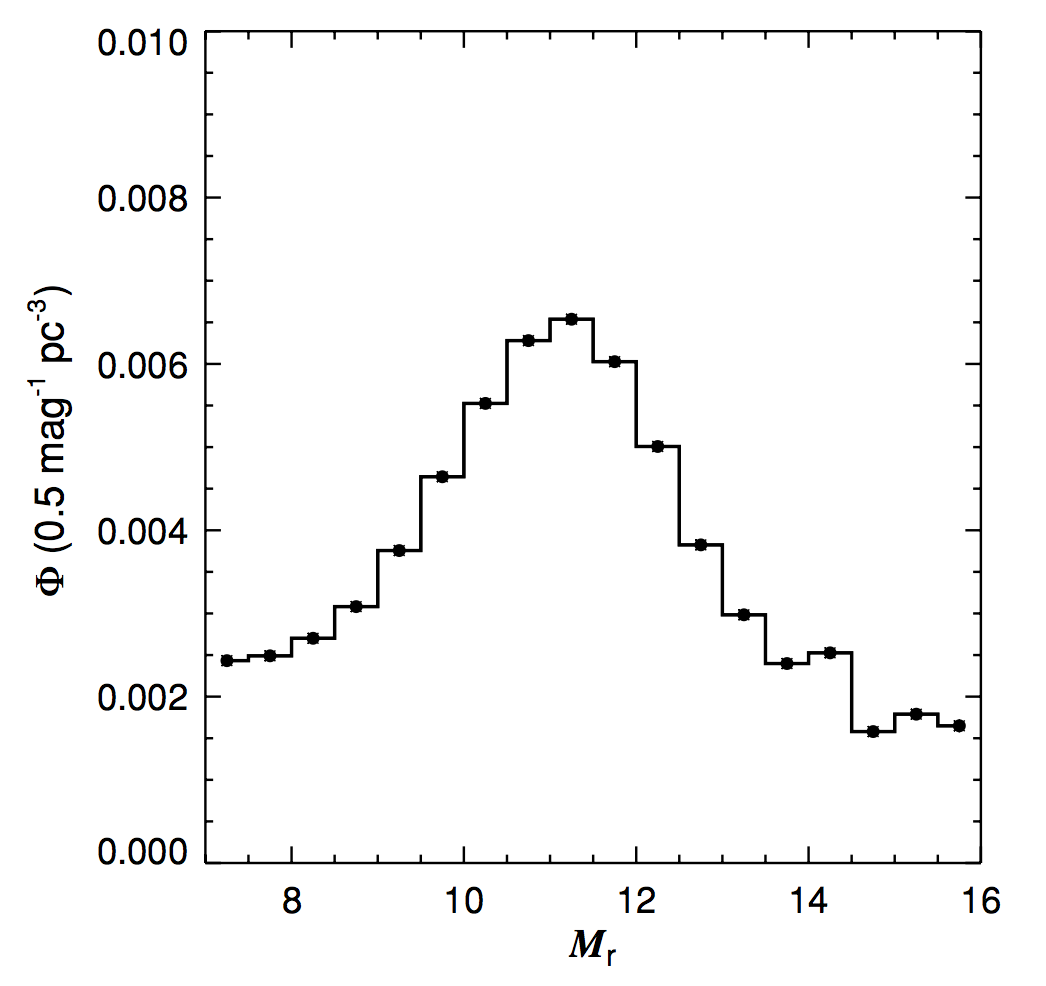
\includegraphics[width=7cm]{figures/lumfunc_before.png} 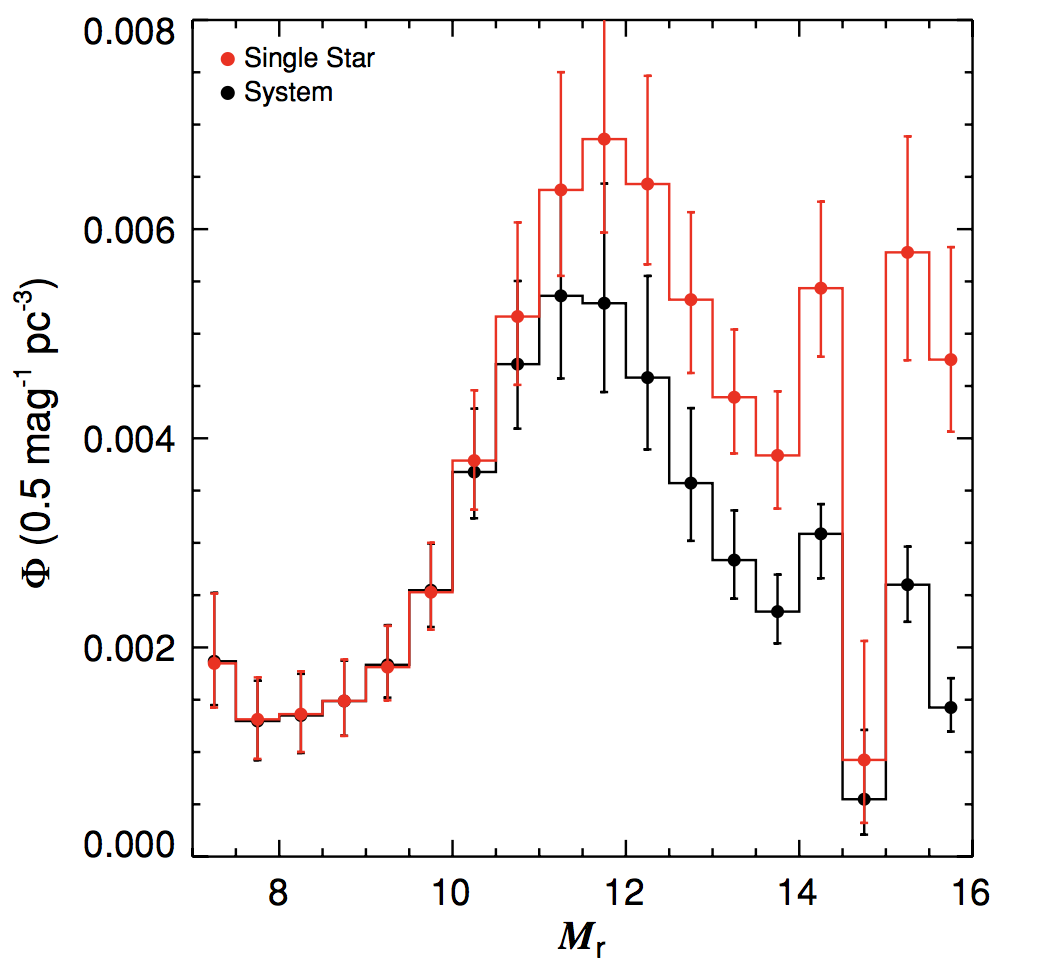
\includegraphics[width=7cm]{figures/lumfunc_after.png}
    \caption{\footnotesize{Luminosity function for MW stars before (left) and after (right) bias correction. Figure taken from Draine (2011).}}
    \label{fig:lumfunc}
\end{figure}

{\noindent}The next step is to convert the luminosity function into a mass function, which requires knowledge of the mass-magnitude relation (MMR) in whatever photometric band we have used for our luminosity function. This must either be determined by theoretical modeling, empirical calibration, or both. Particularly at the low-mass end, the theoretical models tend to have significant uncertainties arising from complex atmospheric chemistry that affects the optical and even NIR colours. For empirical calibrations, the data are only as good as the empirical mass determinations, which must come from orbit modeling. This requires the usual schemes for measuring stellar masses from orbits, e.g., binaries that are both spectroscopic and eclipsing, and thus have known inclinations, or visual binaries with measured radial velocities. 

{\noindent}As with the luminosity function, there are a number of possible biases because the stars are not uniform in either age or metallicity, and as a result there is no true single MMR. This would only introduce a random error if the age and metallicity distribution of the sample used to construct the MMR were the same as that in the IMF survey, but there is no reason to believe that this is actually
the case. The selection function used to determine the empirical mass-magnitude sample is complex and poorly characterized, but
it is certainly biased towards systems closer to the Sun, for example. Strategies to mitigate this are similar to those used to mitigate the corresponding biases in the luminosity function.
Once the mass-magnitude relationship and any bias corrections have been applied, the result is a measure of the field IMF. The results appear to be well-fit by a log-normal distribution or a broken power-law, along the lines of the Chabrier (2005) and Kroupa \& Boily (2002) IMFs.

{\noindent}The strategy we have just described works fine for stars up to $\sim0.7\,{\rm M_\odot}$ in mass. However, it fails with higher mass stars, for one obvious reason: stars with masses larger than this can evolve off the main sequence on timescales comparable to the mean stellar age in the Solar neighborhood. Thus the quantity we measure from this procedure is the present-day mass function (PDMF), not the IMF. Even that is somewhat complicated because stars' luminosities start to evolve non-negligibly even before they leave the main sequence, so there are potential errors in assigning masses based on a MMR calibrated from younger stars.

{\noindent}One option in this case is simply to give up and not say anything about the IMF at higher masses. However, there is another option, which is to try to correct for the bias introduced by stellar evolution. Suppose that we think we know both the star formation history of the region we're sampling, $\dot{M}_*(t)$, and the initial mass-dependent main-sequence stellar lifetime, $t_{MS}(M)$. Let $dN/dM$ be the IMF. In this case, the total number of stars formed of the full lifetime of the galaxy in a mass bin from $M$ to $M+dM$ is

\begin{align*}
    \frac{dN_\mathrm{form}}{dM} = \frac{dN}{dM} \int\limits_{-\infty}^0 \dot{M}_*(t){\rm d}t ~ [{\rm M_\odot^{-1}}]
\end{align*}

{\noindent}where $t=0$ represents the present. In contrast, the number of stars per unit mass still on the main sequence is

\begin{align*}
    \frac{dN_\mathrm{MS}}{dM} = \frac{dN}{dM} \int\limits_{-t_\mathrm{MS}(M)}^0 \dot{M}_*(t){\rm d}t ~ [{\rm M_\odot^{-1}}].
\end{align*}

{\noindent}Thus if we measure the main sequence mass distribution $dN_\mathrm{MS}/dM$, we can correct it to the IMF just by multiplying:

\begin{align*}
    \frac{dN}{dM} \propto \left(\frac{dN_\mathrm{MS}}{dM}\right) \frac{\int\limits_{-t_\mathrm{MS}(M)}^0 \dot{M}_*(t){\rm d}t}{\int\limits_{-\infty}^0 \dot{M}_*(t){\rm d}t} ~ [{\rm M_\odot^{-1}}].
\end{align*}

{\noindent}This simply reduces to scaling the number of observed stars by the fraction of stars in that mass bin that are still alive today.

{\noindent}Obviously this correction is only as good as our knowledge of the star formation history, and it becomes increasingly uncertain as the correction factor becomes larger. Thus attempts to measure the IMF from the galactic field even with age correction are generally limited to masses of no more than a few ${\rm M_\odot}$.

{\noindent}\textit{Young clusters (resolved stars)}: To measure the IMF for more massive stars requires a different technique: surveys of young star clusters. The overall outline of the technique is essentially the same as for the field: construct a luminosity function, correct for biases, then use a mass-magnitude relation to convert to a mass function. However, compared to the field, studying a single cluster offers numerous advantages:

\begin{itemize}
    \item If the population is young enough, then even the most massive stars will remain on the main sequence, so there is no need to worry about correcting from the PDMF to the IMF. Even for somewhat older clusters, one can probe to higher masses than would be possible with the $\sim5\,{\rm Gyr}$ old field population.
    \item The stellar population is generally uniform in metallicity or very close to it, so there are no metallicity biases.
    \item The entire stellar population is at roughly the same distance, so there are no Malmquist or extinction biases. Moreover, in some cases the distance to the cluster is known to better than 10\% from radio parallax -- some young stars flare in the radio, and with radio interferometry it is possible to obtain parallax measurements at much larger distances than would be possible for the same stars in the optical.
    \item Low-mass stars and brown dwarfs are significantly more luminous at young ages, and so the same magnitude limit will correspond to a much lower mass limit, making it much easier to probe into the brown dwarf regime.
\end{itemize}

{\noindent}These advantages also come with some significant costs:


\begin{itemize}
    \item The statistics are generally much worse than for the field. The most populous young cluster that is close enough for us to resolve individual stars down to the hydrogen burning limit is the ONC, and it contains only $\sim10^3-10^4$ stars, as compared to $\sim10^6$ for the largest field surveys.
    \item The MMR that is required to convert an observed magnitude into a mass is much more complex in a young cluster, because a significant fraction of the stars may be pre-main sequence. For such stars, the magnitude is a function not just of the mass but also the age, and one must fit both simultaneously, and with significant theoretical uncertainty. How much of a problem this is depends on the cluster age -- for a $100\,{\rm Myr}$ old cluster like the Pleiades, all the stars have reached the main sequence, while for a $\sim1-2\,{\rm Myr}$ old cluster like Orion, almost none have. However, there is an obvious trade-off here: in a Pleiades-aged cluster, the correction for stars leaving the main sequence is significant, while for an Orion-aged cluster it is negligible.
    \item For the youngest clusters, there is usually significant dust in the vicinity of the stars, which introduces extinction and reddening that is not the same from star to star. This introduces scatter, and also potentially bias because the extinction may vary with position, and there is a systematic variation between position and mass (see next point).
    \item Mass segregation can be a problem. In young clusters, the most massive stars are generally found closer to the center -- whether this is a result of primordial mass segregation (the stars formed there), dynamical mass segregation (they formed elsewhere but sank to the center), the result is the same. Conversely, low mass stars are preferentially on the cluster outskirts. This means that studies must be extremely careful to measure the IMF over the full cluster, not just its outskirts or core; this can be hard in the cluster center due to problems with crowding. Moreover, if the extinction is not spatially uniform, more massive stars toward the cluster center are likely to suffer systematically more extinction that low-mass ones.
    \item Dynamical effects can also be a problem. A non-trivial fraction of O and B stars are observed to be moving with very high spatial velocities, above $50\,{\rm km\,s^{-1}}$. There are known as runaways. They are likely created by close encounters between massive stars in the core of a newly-formed cluster that lead to some stars being ejected at speeds comparable to the orbital velocities in the encounter. Regardless of the cause, the fact that this happens means that, depending on its age and how many ejections occurred, the cluster may be missing some of its massive stars. Conversely, because low-mass stars are further from the center, if there is any tidal stripping, that will preferentially remove low-mass stars.
    \item Binary correction is harder for young stars because the binary fraction as a function of mass is much less well known for young clusters than it is for field stars.
\end{itemize}

{\noindent}Probably the best case for studying a very young cluster is the Orion Nebula Cluster, which is $415\,{\rm pc}$ from the Sun. Its distance is known to a few percent from radio interferometry. It contains several thousand stars, providing relatively good statistics, and it is young enough that all the stars are still on the main sequence. It is close enough that we can resolve all the stars down to the brown dwarf limit, and even beyond. However, the ONC's most massive star is only $38\,{\rm M_\odot}$, so to study the IMF at even higher masses requires the use of more distant clusters within which we can't resolve down to to low masses.

{\noindent}For somewhat older clusters, the best case is almost certainly the Pleiades, which has an age of about $120\,{\rm Myr}$. It obviously has no very massive stars left, but there are still $\sim10\,{\rm M_\odot}$ stars present, and it is also close and very well-studied. The IMF inferred for the Pleiades appears to be consistent with that measured in the ONC.

\subsubsection{Follow-up Questions}

\begin{itemize}
    \item How did Salpeter determine the IMF?
    \item How do you normalize the IMF?
    \item Is the upper or lower limit on mass more important for normalization?
\end{itemize}

% --------------------------------------------------------------
%               2. 
% --------------------------------------------------------------

\newpage
\subsection{Question 2}

Describe the orbits of stars in a galactic disk and in galactic spheroid.

\subsubsection{Short answer}

Answer.

\subsubsection{Additional context}

Additional context.

\begin{itemize}
    \item If we perturb a star in the disk in the z-direction, what happens?
    \item If we perturb a star in the disk in the radial-direction, what happens?
    \item What are the observed quantities in each scenario?
    \item How many integrals of motion are there in the disk?
    \item What symmetry leads to energy conservation?
\end{itemize}


% --------------------------------------------------------------
%               3. 
% --------------------------------------------------------------

\newpage
\subsection{Question 3}

Every now and then a supernova explosion occurs within $3\,\mathrm{pc}$ of the Earth. Estimate how long one typically has to wait for this to happen. Why are newborn stars likely to experience this even when they are much younger than the waiting time you have just estimated?

\subsubsection{Short answer}

Answer.

\subsubsection{Additional context}

Additional context.

% --------------------------------------------------------------
%               4. 
% --------------------------------------------------------------

\newpage
\subsection{Question 4}

Galactic stars are described as a collision-less system. Why? (Don’t forget the influence of gravity.)

\subsubsection{Short answer}

Answer.

\subsubsection{Additional context}

Additional context.

\subsubsection{Follow-up Questions}

\begin{itemize}
    \item What happens when stars collide?
    \item Why choose a cross-section that's larger than the star's radius?
    \item What impact parameter do we need for the stars to end up physically touching (calculate it)?
\end{itemize}

% --------------------------------------------------------------
%               5. 
% --------------------------------------------------------------

\newpage
\subsection{Question 5}

Given that only a tiny fraction of the mass of the interstellar medium consists of dust, why is dust important to the chemistry of the medium and to the formation of stars?

\subsubsection{Short answer}

Answer.

\subsubsection{Additional context}

Additional context.

\subsubsection{Follow-up Questions}

\begin{itemize}
    \item Why is molecular hydrogen (H$_2$) so difficult to detect?
    \item What are other ways in which molecular cloud cores cool?
\end{itemize}

% --------------------------------------------------------------
%               6. 
% --------------------------------------------------------------

\newpage
\subsection{Question 6}

The ISM mainly consists of hydrogen and helium, which are very poor coolants. How, then, do molecular cloud cores ever manage to lose enough heat to collapse and form stars? Why are H
and He such poor coolants?

\subsubsection{Short answer}

Answer.

\subsubsection{Additional context}

Additional context.

% --------------------------------------------------------------
%               7. 
% --------------------------------------------------------------

\newpage
\subsection{Question 7}

The stars in the solar neighbourhood, roughly the $300\,\mathrm{pc}$ around us, have a range of ages, metallicities and orbital properties. How are those properties related?

\subsubsection{Short answer}

Answer.

\subsubsection{Additional context}

Additional context.

% --------------------------------------------------------------
%               8. 
% --------------------------------------------------------------

\newpage
\subsection{Question 8}

What are the main sources of heat in the interstellar medium?

\subsubsection{Short answer}

Answer.

\subsubsection{Additional context}

Additional context.

\subsubsection{Follow-up Questions}

\begin{itemize}
    \item Are there any non-ionization sources of heat in the ISM? (shocks)
    \item How do shock waves heat the gas?
    \item Are shock waves adiabatic?
    \item Where do the x-rays for x-ray photoionization come from?
    \item What phases and temperatures of the ISM apply to each example?
\end{itemize}

% --------------------------------------------------------------
%               9. 
% --------------------------------------------------------------

\newpage
\subsection{Question 9}

Draw an interstellar extinction curve (i.e., opacity), from the X-ray to the infrared. What are the physical processes responsible?

\subsubsection{Short answer}

Answer.

\subsubsection{Additional context}

Additional context.

\subsubsection{Follow-up Questions}

\begin{itemize}
    \item What happens at shorter wavelengths, like gamma rays?
\end{itemize}

% --------------------------------------------------------------
%               10. 
% --------------------------------------------------------------

\newpage
\subsection{Question 10}

What is dynamical friction? Explain how this operates in the merger of a small galaxy into a large one.

\subsubsection{Short answer}

Answer.

\subsubsection{Additional context}

Additional context.

% --------------------------------------------------------------
%               11. 
% --------------------------------------------------------------

\newpage
\subsection{Question 11}

Sketch the SED, from the radio to Gamma, of a spiral galaxy like the Milky Way. Describe the source and radiative mechanism of each feature.

\subsubsection{Short answer}

Answer.

\subsubsection{Additional context}

Additional context.

\subsubsection{Follow-up Questions}

\begin{itemize}
    \item How do the relative heights of the optical/FIR peaks change?
\end{itemize}

% --------------------------------------------------------------
%               12. 
% --------------------------------------------------------------

\newpage
\subsection{Question 12}

How many stars does one expect to find within $100\,\mathrm{pc}$ of the Sun? If all stars are distributed evenly across the galaxy, how many of these will be B spectral type or earlier? How many are younger than $100\,\mathrm{Myrs}$?

\subsubsection{Short answer}

Answer.

\subsubsection{Additional context}

Additional context.

\subsubsection{Follow-up Questions}

\begin{itemize}
    \item Justify the assumptions made and explain why they do not match observations (e.g., number density of stars in the MW is not a flat distribution, the SFR isn't constant etc.).
    \item Where are most B-type and other early-type stars actually found?
    \item How do we know how many stars are in the MW?
    \item How do we measure the IMF?
    \item Are high- or low-mass stars more important to constrain the total number of stars?
    \item How many B stars are visible from your backyard? Are there any star forming regions visible from your backyard?
\end{itemize}

% --------------------------------------------------------------
%               13. 
% --------------------------------------------------------------

\newpage
\subsection{Question 13}

Describe what happens as a cloud starts to collapse and form a star. What is the difference between the collapse and contraction stages? What happens to the internal temperature in both? When does the contraction phase end, and why does the end point depend on the mass of the object?

\subsubsection{Short answer}

Answer.

\subsubsection{Additional context}

Additional context.

\subsubsection{Follow-up Questions}

\begin{itemize}
    \item How do you calculate the Jeans mass?
    \item What happens to the temperature during adiabatic contraction?
    \item Draw a plot of density versus temperature to distinguish between the contracting and collapsing phases.
\end{itemize}

% --------------------------------------------------------------
%               14. 
% --------------------------------------------------------------

\newpage
\subsection{Question 14}

Sketch the rotation curve for a typical spiral galaxy. Show that a flat rotation curve implies the existence of a dark matter halo with a density profile that drops off as $1/r^2$.

\subsubsection{Short answer}

Answer.

\subsubsection{Additional context}

Additional context.

\subsubsection{Follow-up Questions}

\begin{itemize}
    \item What assumptions are made in deriving the $1/r^2$ profile?
\end{itemize}

% --------------------------------------------------------------
%               15. 
% --------------------------------------------------------------

\newpage
\subsection{Question 15}

What thermal phases are postulated to exist in the interstellar medium? Describe the dominant mechanism of cooling for each phase.

\subsubsection{Short answer}

Answer.

\subsubsection{Additional context}

Additional context.

\begin{itemize}
    \item Write down typical temperatures and densities for each phase.
    \item Where do you find each of these phases?
    \item Why don't we see molecular gas (H$_2$) in all of these phases?
    \item Describe what each of these regions might looks like.
    \item How do constituents change between the different thermal phases?
\end{itemize}

% --------------------------------------------------------------
%               16. 
% --------------------------------------------------------------

\newpage
\subsection{Question 16}

Characterize the stellar populations in the following regions: i) the Galactic bulge ii) the Galactic disk, outside of star clusters iii) open star clusters iv) globular clusters v) the Galactic halo vi) a typical elliptical galaxy.

\subsubsection{Short answer}

Answer.

\subsubsection{Additional context}

Additional context.

% --------------------------------------------------------------
%               17. 
% --------------------------------------------------------------

\newpage
\subsection{Question 17}

How can one determine the temperature of a HII region?

\subsubsection{Short answer}

Answer.

\subsubsection{Additional context}

Additional context.

% --------------------------------------------------------------
%               18. 
% --------------------------------------------------------------

\newpage
\subsection{Question 18}

What is the G-dwarf problem in the solar neighborhood?

\subsubsection{Short answer}

Answer.

\subsubsection{Additional context}

Additional context.

\subsubsection{Follow-up Questions}

\begin{itemize}
    \item Is it reasonable to assume that the IMF changes over time? Why?
    \item How much does the mean molecular weight change over cosmological timescales?
    \item What is an appropriate value for the mean molecular weight mu? (i.e., 2 for molecular hydrogen setting limits on formation masses.)
    \item Do we talk about upper mass limits because more massive stars can't exist, or because they don't exist?
\end{itemize}



% --------------------------------------------------------------
%               19. 
% --------------------------------------------------------------

\newpage
\subsection{Question 19}

Describe the general characteristics of spiral structure in galaxies.

\subsubsection{Short answer}

Answer.

\subsubsection{Additional context}

Additional context.

% --------------------------------------------------------------
%               Resources 
% --------------------------------------------------------------

\newpage
\subsection{Resources}

\begin{itemize}
    \item Galaxy Formation, Longair (2008)
    \item Galaxies in the Universe, Sparke \& Gallagher (2007)
    \item Galactic Dynamics, Binney \& Tremaine (2011)
    \item Galaxies: Interactions and Induced Star Formation, Kennicutt, Schweizer \& Barnes (1996)
    \item Stellar Populations, Greggio \& Renzini (2011)
    \item Physics of the Interstellar and Intergalactic Medium, Draine (2011)
    \item Astrophysics of the Interstellar Medium, Maciel (2013)
    \item Notes on Star Formation, Krumholz (2015)
    \item Principles of Star Formation, Bodenheimer (2011)
\end{itemize}

\end{document}
